% Versão com todos os títulos em português.
% Model Card do T2 (INF01017 - Aprendizado de Máquina, UFRGS), em 2 páginas, no formato da Figura 2 de
% Mitchell et al. (2019): seções de texto na coluna da esquerda, Quantitative Analyses na da direita,
% Training Data e Evaluation Data lado a lado e Caveats and Recommendations em largura total no fim.
% Compila com pdfLaTeX (padrão do Overleaf) ou XeLaTeX. As figuras ficam na pasta figuras/.
% Os trechos \pendente{...} marcam o que o grupo ainda precisa escrever.
\documentclass[10pt,a4paper]{article}
\usepackage{iftex}
\ifPDFTeX
  \usepackage[utf8]{inputenc}
  \usepackage[T1]{fontenc}
\fi
\usepackage[brazilian]{babel}
\usepackage{libertine}
\usepackage[a4paper,left=1.5cm,right=1.5cm,top=1.5cm,bottom=1.5cm,footskip=0.6cm]{geometry}
\usepackage{graphicx,booktabs,array,enumitem,xcolor,paracol,eso-pic,tikz,tikzpagenodes,ragged2e}
\usepackage{xurl}
\usepackage[colorlinks=true,urlcolor=linkblue,linkcolor=linkblue]{hyperref}
\definecolor{linkblue}{HTML}{1155CC}
\urlstyle{same}
\definecolor{pendente}{HTML}{B4461B}
\graphicspath{{figuras/}}
\pagestyle{empty}

% Moldura do cartão em cada página, como na Figura 2 do artigo
\AddToShipoutPictureBG{\begin{tikzpicture}[remember picture,overlay]
  \draw[black!60,line width=0.5pt] ([xshift=-8pt,yshift=-8pt]current page text area.south west)
    rectangle ([xshift=8pt,yshift=8pt]current page text area.north east);
\end{tikzpicture}}

\setlength{\parindent}{0pt}
\setlength{\JustifyingParindent}{0pt}
\setlength{\parskip}{0pt}
\setlength{\emergencystretch}{2em}
\setlength{\columnsep}{16pt}
\setlist[itemize]{leftmargin=0.9em,label=\textbullet,topsep=1pt,itemsep=0.5pt,parsep=0pt}
\setlength{\tabcolsep}{2.4pt}

% Título de seção do cartão (negrito, sem numeração, como no artigo)
\newcommand{\secao}[1]{\par\vspace{5pt}{\normalsize\bfseries #1}\par\vspace{1pt}}
% Marcador do que o grupo ainda precisa escrever
\newcommand{\pendente}[1]{{\color{pendente}\itshape[A definir pelo grupo: #1]}}
\newcommand{\nota}[1]{\par\vspace{1pt}{\scriptsize #1\par}\vspace{3pt}}

\begin{document}
\shorthandoff{"}
\small

\begin{center}
{\Large\bfseries Model Card - Detector de Ataques Cardíacos}\par\vspace{2pt}
{\footnotesize Gabriel Pieruccini Knopp (00594975) e Vítor Santana Feijó (00588403)\enspace$\cdot$\enspace
INF01017, UFRGS\enspace$\cdot$\enspace \url{https://github.com/vitorsfeijo/Trabalho_ML}}
\end{center}
\vspace{-4pt}

\columnratio{0.56}
\begin{paracol}{2}

\secao{Detalhes do Modelo}
\begin{itemize}
\item Desenvolvido pelos autores (INF01017, UFRGS), novembro de 2026, v1.0.
\item Regressão Logística com regularização L2 (C = 0,1) e limiar de decisão 0,45, em um Pipeline do scikit-learn: imputação pela mediana, padronização z-score e one-hot encoding (13 atributos clínicos, 22 colunas).
\item Escolhida entre Regressão Logística, KNN e Random Forest (indicados no T1), otimizados com nested CV estratificada (5 folds externos $\times$ 3 internos): Grid Search para Regressão Logística e KNN e Optuna (50 trials) para Random Forest, com o limiar otimizado como hiperparâmetro. Sem restrições de fairness.
\item Código, notebooks e figuras no repositório do cabeçalho. Citação: Knopp, G. P.; Feijó, V. S. \textit{Detector de Ataques Cardíacos} (Regressão Logística, v1.0). INF01017, UFRGS, 2026. Licença: código sob MIT; dados sob CC BY 4.0 (UCI). Contato: Issues do repositório no GitHub.

\end{itemize}

\secao{Uso Pretendido}
\begin{itemize}
\item Criado com a intenção de uso acadêmico ou para suporte a um profissional humano.
\item Não deve ser usado para substituir avaliação médica ou para diagnóstico de pacientes.
\item Projetado para usuários capacitados e formados na área, dando um apoio básico para o problema. 
\end{itemize}

\secao{Fatores}
\begin{itemize}
\item Fatores de avaliação: sexo, faixa etária ($<$ 55 e $\geq$ 55 anos; 55 é a mediana de idade do treino) e a interseção sexo $\times$ faixa etária. A base não tem fatores de instrumentação ou de ambiente que variem entre os pacientes.
\item Outros fatores relevantes, como os relacionados à condição clínica do paciente, não foram avaliados pela ausência de formação médica por parte dos autores.
\end{itemize}

\secao{Métricas}
\begin{itemize}
\item Métrica principal: \textbf{F1-score} da classe positiva (com doença), a mesma do T1. Também são reportados recall e ROC-AUC.
\item Por grupo: \textbf{Taxa de Falsos Positivos} (TFP), \textbf{Taxa de Falsos Negativos} (TFN), \textbf{Taxa de Falsa Descoberta} (TFD) e \textbf{Taxa de Falsa Omissão} (TFO), obtidas da matriz de confusão. Paridade de TFN entre grupos corresponde à Igualdade de Oportunidade; paridade de TFN e TFP, à Igualdade de Chances.
\item Limiar 0,45, escolhido na CV interna (de 0,10 a 0,90, maior F1 médio). Nesse contexto, apesar de ter sido usado o F1 que pesa ambos de forma parecida, é preferível reduzir FN (pacientes com doença classificados como sem doença) a custo de aumentar FP (pacientes sem doença classificados como com doença), pela prioridade de salvar vidas às expensas de realizar testes adicionais inúteis.
\item Incerteza: média $\pm$ desvio padrão nos 5 folds externos; IC 95\% por bootstrap (1000 reamostragens dentro de cada grupo).
\end{itemize}

\vspace{4pt}
\begin{minipage}[t]{0.485\linewidth}
{\normalsize\bfseries Dados de Treinamento}\par\vspace{1pt}
\begin{itemize}
\item Base Cleveland (UCI), versão do Kaggle; 302 pacientes após remover 1 duplicata.
\item Treino: 241 pacientes (80\%, estratificado), 110 com doença: mulheres 79 (20), homens 162 (90), $<$ 55 anos 114 (36), $\geq$ 55 anos 127 (74).
\item Alvo: 1 = com doença; ca = 4 e thal = 0 como ausentes.
\end{itemize}
\end{minipage}\hfill
\begin{minipage}[t]{0.485\linewidth}
{\normalsize\bfseries Dados de Avaliação}\par\vspace{1pt}
\begin{itemize}
\item Teste: 61 pacientes (20\%, reservados desde o T1), 28 com doença; usado uma única vez.
\item Predições fora da amostra da nested CV para os 241 pacientes de treino.
\item Mesmo pipeline, ajustado só no treino. Não há base externa.
\end{itemize}
\end{minipage}

\secao{Considerações Éticas}
\begin{itemize}
\item Dados de saúde e sexo dos pacientes, anonimizados na base original da UCI. 
\item Se o modelo for utilizado corretamente, poderá ajudar a preservar vidas humanas, mas jamais pode substituir a tomada de decisão por parte do profissional humano, nem eximir a sua responsabilidade.
\end{itemize}

\switchcolumn

\secao{Análises Quantitativas}
\centering
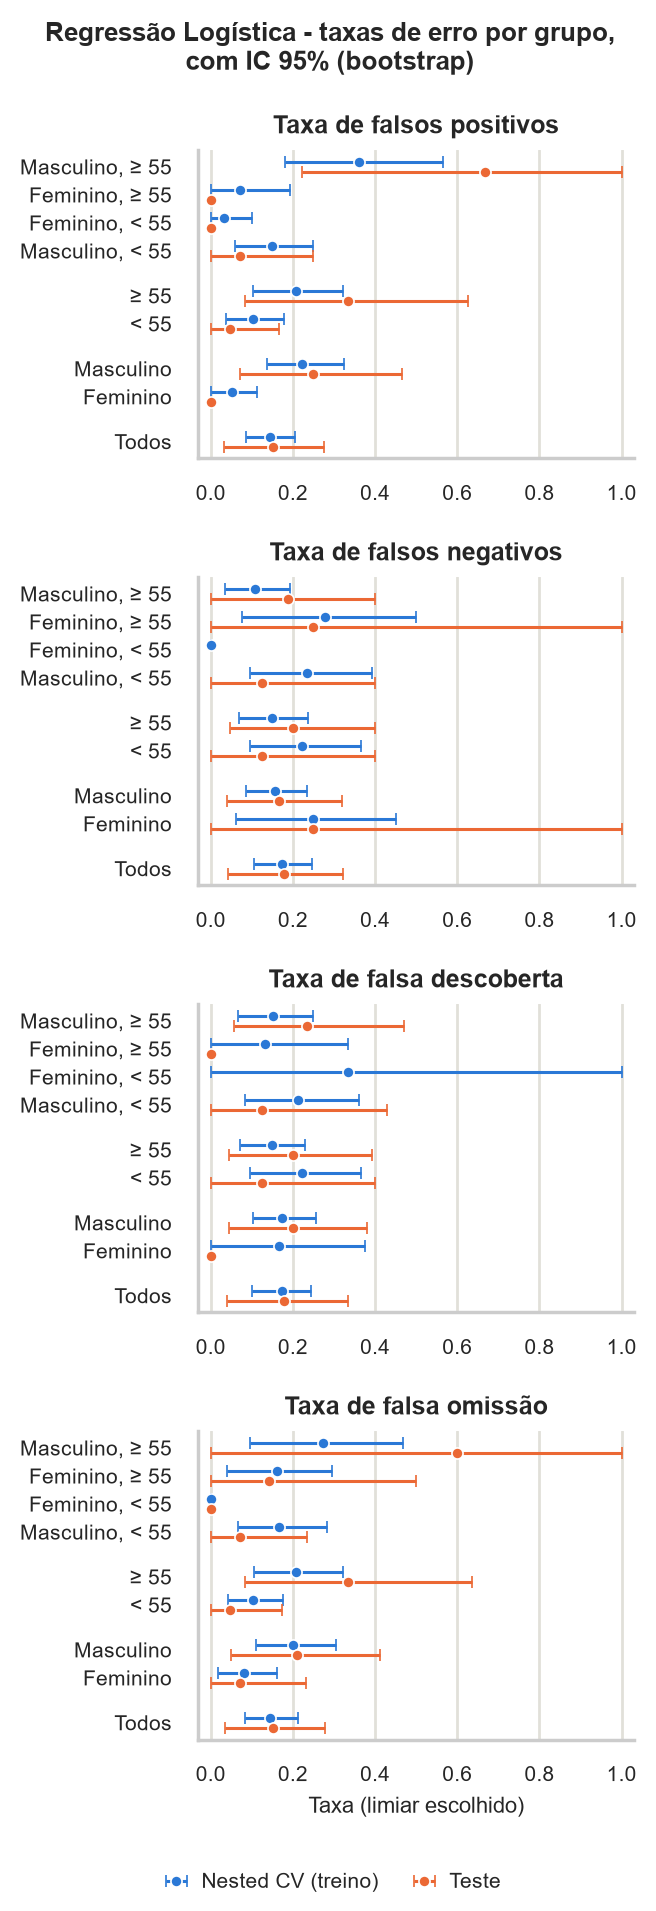
\includegraphics[width=\linewidth,height=0.79\textheight,keepaspectratio]{t2_taxas.png}\par
\justifying
\nota{Regressão Logística no limiar escolhido. Pontos: valor; barras: IC 95\% (bootstrap). Azul: nested CV (241 pacientes de treino); laranja: teste (61). Taxas indefinidas (grupo sem doentes) não aparecem.}

\end{paracol}
\newpage

\secao{Análises Quantitativas (continuação)}
\footnotesize % página 2 em 8 pt para caber no limite de 2 páginas
\columnratio{0.56}
\begin{paracol}{2}
{\footnotesize\bfseries Seleção do modelo}\par\vspace{1pt}
{\footnotesize \begin{tabular}{@{}l c c c c c@{}}
\toprule
Modelo & Limiar & F1 nested CV & F1 teste & Recall teste & ROC-AUC teste \\
\midrule
\textbf{Regressão Logística} & 0,45 & 0,827 $\pm$ 0,058 & \textbf{0,821} & 0,821 & 0,922 \\
KNN & 0,45 & 0,811 $\pm$ 0,040 & 0,800 & 0,786 & 0,893 \\
Random Forest & 0,50 & 0,808 $\pm$ 0,039 & 0,755 & 0,714 & 0,883 \\
\bottomrule
\end{tabular}}
\nota{Nested CV: média $\pm$ desvio padrão nos 5 folds externos. Teste: modelo final de cada algoritmo, avaliado uma única vez. Curvas ROC e Precisão-Recall ao lado.}
\begin{itemize}
\item Em geral, a Regressão Logística teve melhor desempenho em todas as métricas primárias avaliadas, com F1, recall e ROC-AUC mais altos no teste. KNN teve desempenho intermediário e Random Forest, pior dentre os 3. Além disso, a Regressão Logística é inerentemente interpretável, e, assim, foi escolhida como modelo final. Ademais, como a regressão logística é linear, isso sugere que a modelagem do espaço do problema, provavelmente, seja linear, e, por isso, a complexidade dos outros modelos não trouxe ganhos de desempenho.
\end{itemize}

\vspace{4pt}
{\footnotesize\bfseries Falsos negativos por grupo (Regressão Logística)}\par\vspace{1pt}
{\footnotesize \begin{tabular}{@{}l c c c c@{}}
\toprule
 & \multicolumn{2}{c}{Nested CV (treino)} & \multicolumn{2}{c}{Teste} \\
\cmidrule(lr){2-3}\cmidrule(l){4-5}
Grupo & FN/doentes & TFN [IC 95\%] & FN/doentes & TFN [IC 95\%] \\
\midrule
Todos & 19/110 & 0,17 [0,10; 0,25] & 5/28 & 0,18 [0,04; 0,32] \\
\addlinespace[1.5pt]
Fem. & 5/20 & 0,25 [0,06; 0,45] & 1/4 & 0,25 [0,00; 1,00] \\
Masc. & 14/90 & 0,16 [0,09; 0,23] & 4/24 & 0,17 [0,04; 0,32] \\
\addlinespace[1.5pt]
$<$ 55 & 8/36 & 0,22 [0,10; 0,37] & 1/8 & 0,12 [0,00; 0,40] \\
$\geq$ 55 & 11/74 & 0,15 [0,07; 0,24] & 4/20 & 0,20 [0,05; 0,40] \\
\addlinespace[1.5pt]
Fem., $<$ 55 & 0/2 & 0,00 [0,00; 0,00] & --/0 & \textit{indef.} \\
Fem., $\geq$ 55 & 5/18 & 0,28 [0,08; 0,50] & 1/4 & 0,25 [0,00; 1,00] \\
Masc., $<$ 55 & 8/34 & 0,24 [0,10; 0,39] & 1/8 & 0,12 [0,00; 0,40] \\
Masc., $\geq$ 55 & 6/56 & 0,11 [0,03; 0,19] & 3/16 & 0,19 [0,00; 0,40] \\
\midrule
\textit{Diferença de TFN} & \multicolumn{2}{c}{[IC 95\%]} & \multicolumn{2}{c}{[IC 95\%]} \\
Fem. $-$ Masc. & \multicolumn{2}{c}{0,09 [-0,09; 0,30]} & \multicolumn{2}{c}{0,08 [-0,29; 0,58]} \\
$\geq$ 55 $-$ $<$ 55 & \multicolumn{2}{c}{-0,07 [-0,23; 0,08]} & \multicolumn{2}{c}{0,07 [-0,22; 0,35]} \\
Fem., $<$ 55 $-$ Masc., $<$ 55 & \multicolumn{2}{c}{-0,24 [-0,38; -0,12]} & \multicolumn{2}{c}{\textit{indef.}} \\
Fem., $\geq$ 55 $-$ Masc., $\geq$ 55 & \multicolumn{2}{c}{0,17 [-0,04; 0,39]} & \multicolumn{2}{c}{0,06 [-0,31; 0,56]} \\
\bottomrule
\end{tabular}}
\nota{FN: pacientes com doença classificados como sem doença; TFN = FN/doentes. Diferença de TFN entre grupos do mesmo fator: 0 corresponde à Igualdade de Oportunidade; IC 95\% por bootstrap. indef.: grupo sem doentes. Com apenas 2 doentes em Fem., $<$ 55, o IC desse grupo e o da sua diferença não são confiáveis.}
\centering
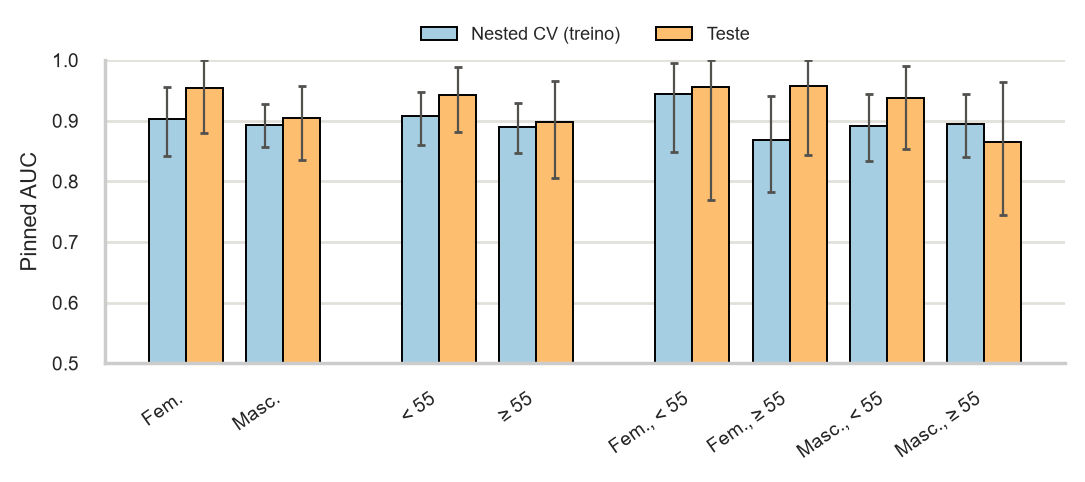
\includegraphics[width=0.8\linewidth]{t2_pinned_auc.png}\par
\justifying
\nota{Pinned AUC: AUC do grupo combinado com uma amostra de mesmo tamanho de toda a base de avaliação (média e IC 95\% de 1000 reamostragens).}
\begin{itemize}
\item Inicialmente, destaca-se a pouca representatividade de alguns grupos e intersecções, como Fem., $<$ 55 (2 doentes no treino e nenhum no teste) e Fem., $\geq$ 55 (18 doentes no treino e 4 no teste). Isso gera ICs amplos, que incluem 0, e dificulta a avaliação de paridade entre os grupos.
\item Ademais, o grupo com menor taxa de falso negativo no Nested CV são os homens com 55 anos ou mais, pela sua alta representatividade nos dados de treinamento.
\item Já no teste, em contrapartida, homens com menos de 55 anos apresentam as taxas de falso negativo mais baixas, o que pode ser, possivelmente, em decorrência da amostragem dos dados originais - se uma pessoa mais jovem foi entrevistada e teve seus dados coletados, ela, talvez, já apresentava algum sintoma relacionado (pode não ter sido interessante "encher" a base de dados com pessoas saudáveis), gerando um certo viés.
\end{itemize}

\switchcolumn
\centering
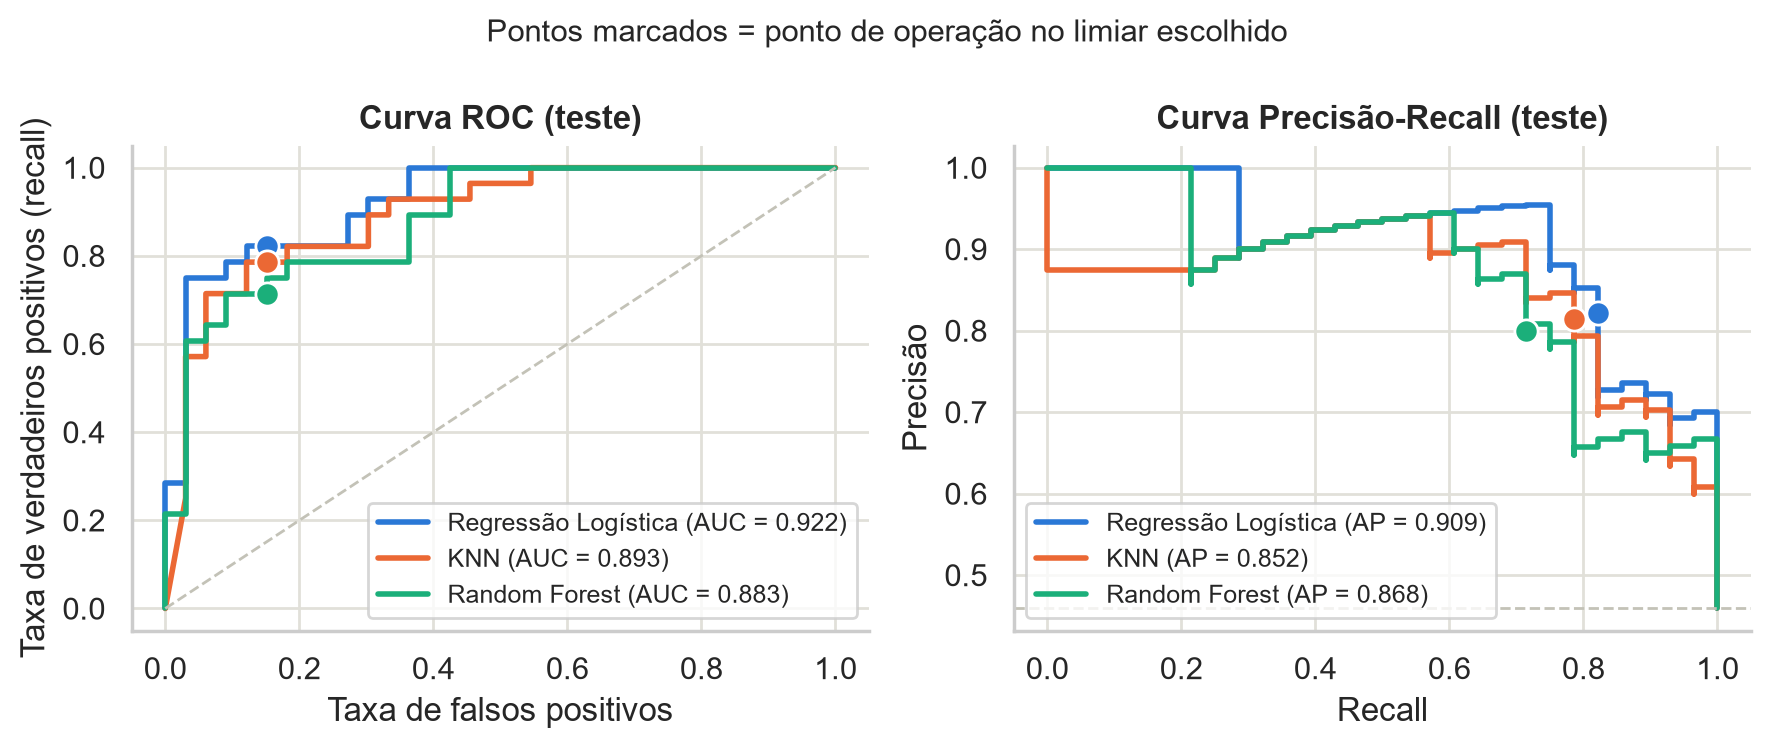
\includegraphics[width=\linewidth]{t2_roc_pr.png}\par
\justifying
\nota{Curvas ROC e Precisão-Recall no teste; pontos = ponto de operação de cada modelo no limiar escolhido.}

\vspace{3pt}
{\footnotesize\bfseries Análise de erros (Regressão Logística)}\par\vspace{1pt}
\begin{itemize}
\item Classe mais difícil: \textbf{com doença}. A taxa de erro entre os doentes (TFN) é um pouco maior que entre os saudáveis (TFP): 0,17 contra 0,15 na nested CV (19/110 e 19/131) e 0,18 contra 0,15 no teste (5/28 e 5/33). A diferença é pequena: no teste, ela desaparece com um paciente a mais ou a menos.
\item Amostras ``confusas'': os FN se parecem com os pacientes sem doença (VN) - thalach médio de 155 bpm (VN 160; VP 136), oldpeak 0,7 (VN 0,5; VP 1,8), ca $\geq$ 1 em 29\% (VN 16\%; VP 75\%) e thal normal em 71\% (VN 86\%; VP 17\%). Os FP se aproximam dos doentes - 88\% homens (VP 84\%), com ca $\geq$ 1 em 38\% e thal normal em 33\%. Erros com alta confiança (probabilidade $<$ 0,25 nos FN e $>$ 0,75 nos FP) - 7 FN e 4 FP na nested CV; 1 FN e 1 FP no teste.
\nota{Médias e proporções de nested CV e teste juntos (302 pacientes); VP e VN: acertos com e sem doença.}
\end{itemize}

\vspace{4pt}
{\footnotesize\bfseries Interpretabilidade (Regressão Logística)}\par\vspace{1pt}
\centering
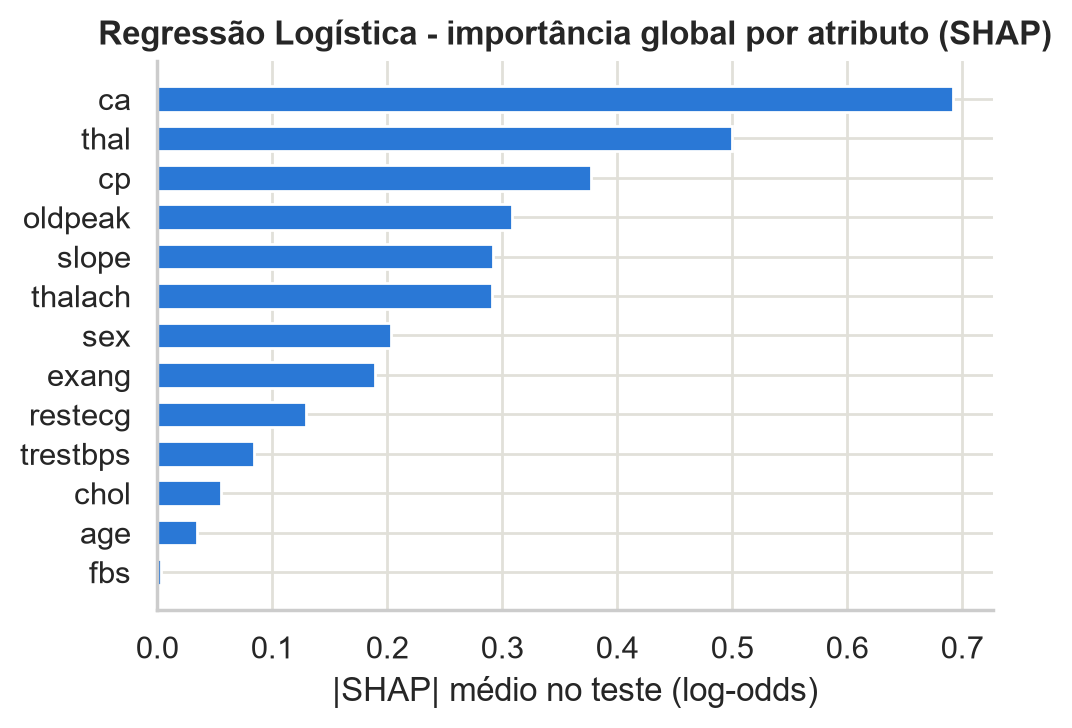
\includegraphics[width=0.66\linewidth]{t2_shap.png}\par
\nota{SHAP (LinearExplainer) no teste: média de |SHAP| por atributo original.}
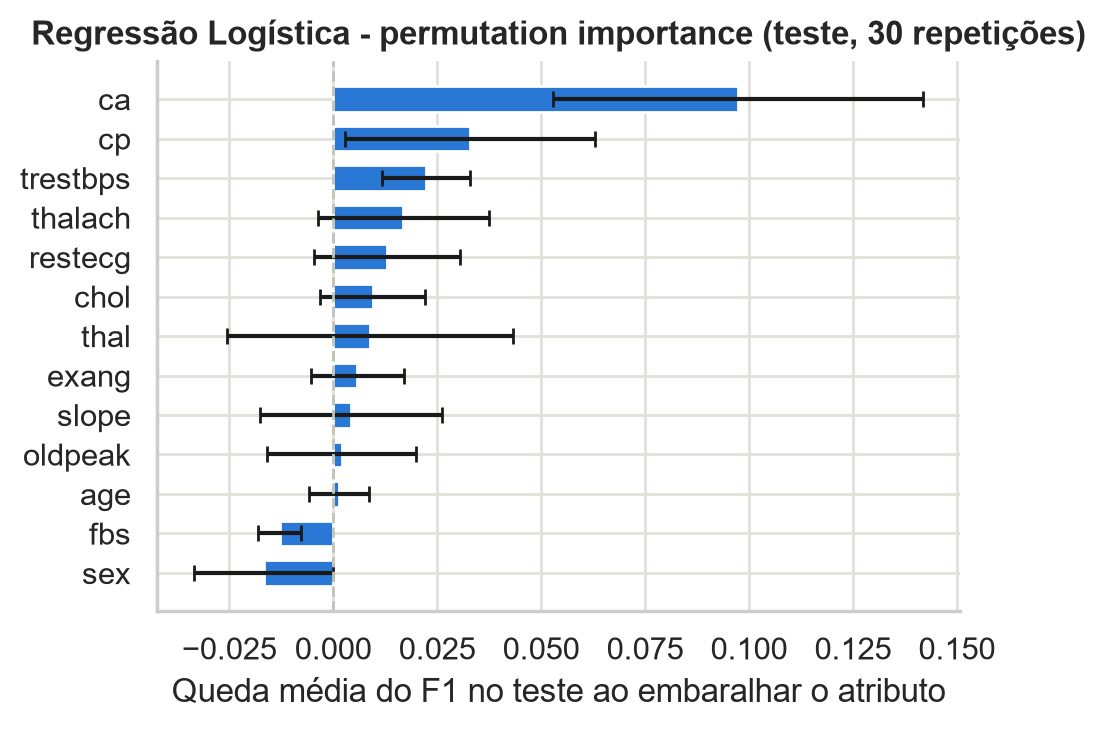
\includegraphics[width=0.66\linewidth]{t2_permutacao.png}\par
\justifying
\nota{Permutation importance no teste: queda média do F1 ao embaralhar cada atributo (30 repetições), com desvio padrão.}
\begin{itemize}
\item Analisando a importância dos atributos pelos algoritmos de interpretabilidade, percebemos que idade é dada como pouco importante para o modelo (pouco usada), mas isso pode ser explicado pelo fato dos atributos relativos à saúde do paciente servirem/atuarem como proxies, já que a informação contida em idade (mais velho = maior chance de doença) também é contida em atributos como thalach (batimento cardíaco máximo) e ca (número de vasos principais coloridos na fluoroscopia), já que, conforme passa a idade, a saúde do paciente vai naturalmente se deteriorando, o que afeta os atributos mencionados.
\item Novamente, devido à falta de conhecimento médico dos autores, não foi possível afirmar que o modelo aprendeu padrões que fazem sentido clinicamente ou não.
\end{itemize}

\end{paracol}

\secao{Ressalvas e Recomendações}
\begin{itemize}
\item É recomendada extrema cautela ao utilizar o modelo em um contexto médico, já que ele foi treinado com uma base de dados extremamente pequena, e com alguns grupos muito pouco representados.
\item Antes de qualquer uso prático do modelo, é essencial que ele seja testado em mais datasets, e que seja feito um monitoramento contínuo de seu desempenho, com supervisão humana profissional.
\item Para o modelo funcionar de forma ideal, a base de dados deve possuir todos os atributos envolvidos dos pacientes (que tenham sido previamente examinados) e que suas classes sejam minimamente balanceadas.
\end{itemize}

\vfill
{\scriptsize Referências: Bhat, N. \textit{Health care: Data set on Heart attack possibility} (Kaggle); Janosi, A. et al. \textit{Heart Disease} (UCI ML Repository, 1988); Dixon, L. et al. \textit{Measuring and Mitigating Unintended Bias in Text Classification} (AIES '18); Mitchell, M. et al. \textit{Model Cards for Model Reporting} (FAT* '19).\par}
\end{document}
